\documentclass[11pt]{article}

\usepackage[a4paper,margin=1in]{geometry}
\usepackage[T1]{fontenc}
\usepackage[utf8]{inputenc}
\usepackage{lmodern}
\usepackage{microtype}
\usepackage{amsmath,amssymb}
\usepackage{booktabs}
\usepackage{array}
\usepackage{enumitem}
\usepackage{graphicx}
\usepackage{float}
\usepackage[hidelinks]{hyperref}
\usepackage[numbers]{natbib}
\usepackage{caption}

\setlength{\parskip}{0.35em}
\setlength{\parindent}{0pt}
\renewcommand{\arraystretch}{1.12}

\title{Protocol-Dependent Non-Portability of Self-Reported Confidence in English-to-German Machine Translation Across Providers}
\author{Umberto Altieri}
\date{}

\begin{document}
\maketitle

\begin{abstract}
This paper studies whether self-reported confidence behaves as a portable decision signal in English-to-German machine translation when a schema-equivalent prompting protocol is applied across multiple LLM providers. Eight models from OpenAI, Anthropic, and Google are evaluated with temperature 0 on 500 sentences from WMT17, yielding 4,000 translation--confidence pairs. Translation quality is scored with sentence-level chrF, and low-quality cases are operationally defined as the bottom 20\% of chrF scores within each model. Relative to that operational label, the paper reports expected calibration error (ECE) as a comparative alignment diagnostic and mismatch@0.9 as a fixed-threshold operating-point statistic. Mean chrF is relatively similar across models (54.0--60.1), but the confidence operating points are not: within-model ECE ranges from 0.076 (GPT-5-nano) to 0.180 (Gemini 2.5 Pro), and mismatch@0.9 ranges from 0.2\% to 18.2\%. A lightweight source-side surface-complexity proxy is examined only as a secondary descriptive stratification signal, and its relationship to confidence is weak. The main conclusion is practical and explicitly scoped to this setup: under this protocol and chrF-based target, prompt-elicited confidence should not be treated as a portable probability across providers, and a shared threshold such as $\tau = 0.9$ does not induce comparable operating points even when average chrF is similar. A supplementary held-out isotonic analysis shows that lightweight post-hoc calibration can reduce ECE for most models, but the required mappings remain provider-specific. A secondary metric-robustness check using the strongest metric available in the current environment preserves the same qualitative portability conclusion. The paper does not evaluate calibration to semantic correctness directly, and low mismatch at a strict threshold can reflect either useful separation or simple conservatism. Code, prompts, and generated artifacts are released to support reproducible multi-provider MT reliability comparisons.
\end{abstract}

\section{Introduction}

Large language models (LLMs) are increasingly used as machine translation systems. In many deployment settings, average translation quality is not enough: a usable system also needs a signal that helps decide when an output should be trusted, routed for review, or deferred. For closed-source APIs, prompting the model to output a scalar confidence is attractive because it is simple, model-agnostic, and inexpensive. Recent work on LLM confidence estimation, however, shows that prompt-elicited or verbalized confidence is often miscalibrated, prompt-sensitive, and difficult to compare across settings \citep{geng-etal-2024-survey,yang2024verbalizedconfidence,wang2024calibratingverbalized,liu2025uqsurvey}.

This paper studies that problem in a controlled English-to-German MT setting and focuses on a narrower question than general confidence estimation: whether prompt-elicited, self-reported confidence is comparable enough across providers to support fixed decision policies such as abstention or human routing. This is a practically relevant question because deployment policies often treat confidence as a shared scalar interface: if different providers emit values in the same nominal range $[0,1]$, it is natural to ask whether a common threshold can be reused across systems under a shared prompting protocol. The protocol used here is schema-equivalent and semantically standardized across OpenAI, Anthropic, and Google Gemini model families, but not literally identical word-for-word across providers. For each source sentence, the pipeline collects (i) a translation and (ii) a post-hoc confidence score conditioned on the source and the model output. Confidence is then evaluated against a reproducible reference-based quality signal and, secondarily, against a lightweight source-side surface-complexity proxy.

The key construct in this paper is operational rather than semantic. The analysis does not use human judgments of correctness. Instead, it defines a low-quality event through sentence-level chrF quantiles and asks whether self-reported confidence tracks that event under a shared protocol. The resulting comparisons are therefore about the portability of confidence relative to a reproducible chrF-based target, not about direct calibration to semantic correctness. This distinction matters throughout: the paper is strongest when read as a comparison of fixed-threshold operating points across providers rather than as a complete account of confidence utility.

The analysis addresses two questions:
\begin{enumerate}[leftmargin=*]
\item \textbf{Comparative alignment under an operational low-quality definition:} how do self-reported confidence scores align with a reproducible chrF-based low-quality event when that event is defined by quantiles?
\item \textbf{Provider portability under a fixed threshold:} how often do high-confidence low-quality outputs occur under a shared threshold, and does this rate vary across source-side surface-complexity strata?
\end{enumerate}

The main result is practical rather than theoretical. Models with similar mean chrF differ substantially in ECE and in the rate at which they assign high confidence to low-quality outputs at strict thresholds. A fixed policy such as ``route to a human if confidence $< 0.9$'' is therefore not portable across providers without calibration or threshold tuning. At the same time, low mismatch at a strict threshold does not by itself prove superior selective utility, because a conservative model can also look safer simply by rarely emitting values above that threshold. The surface-complexity analysis is more modest: it is included as a secondary stratification analysis rather than as a validated model of translation difficulty \citep{yang2024verbalizedconfidence,wang2024calibratingverbalized,xue-etal-2025-mlingconf}.

\paragraph{Contributions.}
\begin{itemize}[leftmargin=*]
\item A unified, reproducible pipeline for multi-provider MT evaluation with self-reported confidence, covering prompts, parsing, metrics, analysis, and plots.
\item An empirical comparison of ECE and high-confidence low-quality mismatch across eight LLMs from three providers under a shared English-to-German MT protocol, framed as a comparison of provider-specific operating points relative to a reproducible chrF-based target.
\item A secondary stratified analysis using a lightweight source-side surface-complexity proxy, included explicitly as a coarse descriptive analysis rather than a validated measure of translation difficulty.
\end{itemize}

\section{Related work}

\paragraph{MT evaluation, quality estimation, and reliability signals.}
Automatic MT evaluation has long relied on overlap-based metrics such as BLEU and its standardized variants \citep{post2018bleu}, as well as character-level metrics such as chrF \citep{popovic2015chrf}. Learned metrics, including COMET and BLEURT, generally correlate better with human judgments \citep{rei2020comet,sellam2020bleurt}. More recent work has continued to strengthen this line: xCOMET adds fine-grained error detection on top of sentence-level scoring \citep{guerreiro-etal-2024-xcomet}, and the WMT24 Metrics Shared Task specifically examined how metrics behave on LLM-generated translations \citep{freitag-etal-2024-llms}. Quality estimation (QE) predicts translation quality without references and remains an active WMT shared-task line \citep{specia2018wmtqe,zerva-etal-2024-findings}. MT confidence estimation itself is also a longstanding topic rather than a new LLM-era concern: early work studied sentence-level and word-level confidence estimation for MT outputs well before contemporary API-based systems \citep{blatz-etal-2004-confidence}. This paper does not propose a new QE or confidence-estimation model; it studies a narrower reliability signal emitted by the generating model itself.

\paragraph{LLM-based MT evaluation and uncertainty-aware MT reliability.}
Recent work has also studied whether LLMs can serve as MT evaluators and what information they need to do so reliably \citep{qian-etal-2024-what}. This literature is relevant because it frames translation reliability as a prediction problem, but it typically studies external evaluation signals rather than self-reported confidence from the model that produced the translation. Closer in spirit are confidence-aware MT reliability approaches that attach uncertainty estimates to translation quality prediction, including recent confidence-aware QE models such as Early-Exit and Instant Confidence COMET \citep{zouhar-etal-2026-early}. Relative to that line, the present paper asks a narrower black-box question: whether the self-reported confidence already exposed through a shared API-style interaction is stable enough across providers to support common threshold policies.

\paragraph{Uncertainty, calibration, and selective prediction.}
Modern neural networks are often miscalibrated \citep{guo2017calibration}. Calibrated probabilities are useful for selective prediction or abstention policies, where a system chooses when to defer \citep{geifman2017selective}. Classical approaches estimate uncertainty through approximate Bayesian methods such as MC dropout \citep{gal2016dropout} or deep ensembles \citep{lakshminarayanan2017simple}, followed by post-hoc calibration \citep{kuleshov2018accurate}. For LLMs, the literature has expanded rapidly: recent surveys synthesize the challenges of confidence estimation and calibration for generated text, especially in black-box settings where access to logits is unavailable or impractical \citep{geng-etal-2024-survey,liu2025uqsurvey}. Black-box calibration methods that use only textual generations are particularly relevant here because they match the interface available in many provider APIs \citep{ulmer-etal-2024-calibrating}.

\paragraph{Verbalized confidence and self-evaluation in LLMs.}
Prior work suggests that language models can sometimes assess the validity of their own outputs when asked in the right format \citep{kadavath2022language}. More recent work studies verbalized confidence directly: Yang et al.\ show that such scores can be useful but are highly prompt-dependent \citep{yang2024verbalizedconfidence}, while Wang et al.\ analyze how post-hoc calibration can improve verbalized probability estimates for black-box models \citep{wang2024calibratingverbalized}. Yona et al.\ further show that models often fail to express intrinsic uncertainty faithfully in words, which is directly relevant when a scalar confidence is elicited through natural-language instructions rather than read from model internals \citep{yona-etal-2024-large}. In multilingual settings, MlingConf shows that confidence estimation itself can vary across languages and prompting conditions \citep{xue-etal-2025-mlingconf}.

Relative to QE, uncertainty-aware MT evaluation, and LLM-as-evaluator work, the present paper studies a narrower but practically distinct signal: the self-reported confidence emitted by the same black-box model that produced the translation. That signal is weaker than an external evaluator in principle, but it is attractive in deployment because it is immediate, cheap, and provider-agnostic at the API level. The question addressed here is therefore not whether self-reported confidence is the best possible reliability estimator, but whether it is stable enough across providers to support shared threshold policies under a single prompt protocol. The results suggest that, under the protocol and target used here, it is not.

\section{Experimental setup}

\subsection{Dataset}
The experiments use the WMT17 English-to-German test set \citep{bojar2017wmt17}, accessed through \texttt{sacrebleu} \citep{post2018bleu}. From the full test set, 500 sentence pairs are sampled with a fixed random seed (123) and stored as JSONL records containing \texttt{id}, \texttt{src}, and \texttt{ref}. A 500-sentence sample was chosen to keep the multi-provider evaluation financially and operationally tractable while still producing 4,000 total model outputs for comparative analysis.

\subsection{Models and providers}
Eight LLMs across three providers are evaluated: OpenAI (GPT-5.2, GPT-5-mini, GPT-5-nano), Anthropic (Claude Opus 4.6, Claude Sonnet 4.5, Claude Haiku 4.5), and Google (Gemini 2.5 Pro, Gemini 2.5 Flash). Each model is queried on the same 500 inputs. In the canonical artifact snapshot used here, all models contribute 500 usable confidence values for 500 total inputs, as reported in Table~\ref{tab:main}. The accompanying materials record the exact provider model identifiers used in the canonical runs so that the reported comparisons remain tied to a specific released snapshot rather than to shifting provider aliases in the abstract.

\subsection{Prompting protocol}
Each input sentence triggers two calls:
\begin{enumerate}[leftmargin=*]
\item \textbf{Translation:} English-to-German translation, returned as a strict JSON object with key \texttt{translation}.
\item \textbf{Confidence:} a scalar confidence in $[0,1]$, returned as a strict JSON object with key \texttt{confidence}, conditioned on the source sentence and the model translation rather than the human reference.
\end{enumerate}
All runs use temperature 0 and provider-side output limits fixed in advance within the shared evaluation protocol. These limits serve to standardize response formatting and generation budget across providers rather than to define a substantive experimental variable. The prompts are schema-equivalent across providers, but Anthropic uses slightly shorter wording while preserving the same required JSON fields. When outputs are malformed or missing required fields, the pipeline applies deterministic extraction and repair heuristics documented in Appendix~\ref{app:prompts} and in the accompanying reproducibility package. Latency and token usage are logged whenever the provider SDK exposes them. Because latency is measured through live provider APIs, it should be interpreted as deployment-facing wall-clock behavior under the recorded runs rather than as a pure model-intrinsic efficiency measure.

\subsection{Pipeline and artifacts}
The pipeline consists of dataset creation, model calls, feature extraction and metric computation, aggregation, and analysis/plot generation. The accompanying reproducibility package includes prompts, configuration files, generated figures and tables, and the metadata needed to regenerate the reported outputs.

\section{Methods}

\subsection{Reference-based quality}
Each translation is scored against the reference using sentence-level chrF \citep{popovic2015chrf} as the main quality signal, computed with \texttt{sacrebleu} \citep{post2018bleu}. chrF is inexpensive, easy to reproduce, and still widely used in WMT-style evaluation. Learned metrics such as COMET, BLEURT, and xCOMET often correlate better with human judgments, especially when finer-grained error analysis is needed \citep{rei2020comet,sellam2020bleurt,guerreiro-etal-2024-xcomet,freitag-etal-2024-llms}. This paper nevertheless uses chrF as the primary metric because the aim is to study cross-provider confidence behavior under a lightweight and fully reproducible reference-based protocol. Sentence-level BLEU is also computed by the pipeline, but the submitted robustness appendix reports only the chrF-based exports available in the released snapshot used for this paper.

\subsection{Source-side surface-complexity proxy}
A lightweight source-side surface-complexity score is computed from surface features that do not require model internals:
\begin{itemize}[leftmargin=*]
\item \textbf{Length:} number of whitespace tokens (\texttt{src\_len\_tokens});
\item \textbf{Depth-like heuristic:} a capped function of length ($\texttt{syntactic\_depth} \approx \min(10, \lfloor \texttt{len}/4 \rfloor + 1)$);
\item \textbf{Lexical rarity ratio:} fraction of tokens with length $\ge 8$ (\texttt{rare\_ratio});
\item \textbf{Name proxy:} count of capitalized tokens (\texttt{ner\_count}).
\end{itemize}
Each feature is z-scored across all sentences and summed:
\[
\mathrm{complexity}(x)=z(\mathrm{len})+z(\mathrm{depth})+z(\mathrm{rare})+z(\mathrm{names}).
\]
Each example is then assigned to a surface-complexity quartile (Q1 lowest complexity to Q4 highest complexity) using the empirical quartiles of this score. This proxy is intentionally shallow and is used only for stratified descriptive analysis; it is not a validated measure of translation difficulty. In particular, the depth-like term is a coarse length-derived heuristic rather than an independent syntactic analysis.

\subsection{Operational low-quality definitions}
To study calibration and thresholded mismatch using a reproducible binary target, a low-quality event is defined by a quantile threshold on sentence-level chrF:
\begin{itemize}[leftmargin=*]
\item \textbf{Within-model low-quality cases:} for each model, mark the lowest 20\% chrF examples as low quality.
\item \textbf{Global low-quality cases:} mark the lowest 20\% chrF examples across all models as low quality.
\end{itemize}
Unless stated otherwise, results use the within-model low-quality definition. Under this definition, low-quality prevalence is fixed at 20\% within each model by construction. The resulting target is therefore a relative quality event rather than an absolute error rate, and it should not be read as a direct measure of semantic incorrectness. The main reason for using this target is comparability across providers under a reproducible reference-based protocol, not the claim that the bottom-20\% boundary has intrinsic semantic status.

\subsection{Calibration and reliability diagrams}
Expected calibration error (ECE) is computed with $B=10$ confidence bins, where bin accuracy is defined as the fraction of non-low-quality outputs under the chrF-based operational label:
\[
\mathrm{ECE}=\sum_{b=1}^{B}\frac{|S_b|}{N}\left|\mathrm{acc}(S_b)-\mathrm{conf}(S_b)\right|,
\]
where $\mathrm{acc}(S_b)$ is the fraction of non-low-quality outputs in bin $b$ and $\mathrm{conf}(S_b)$ is the mean confidence in that bin \citep{guo2017calibration}. In this paper, ECE therefore measures alignment between self-reported confidence and a reproducible chrF-based low-quality event, not direct calibration to semantic correctness. Because the within-model label fixes non-low-quality prevalence at 80\%, ECE should be read as a comparative alignment diagnostic rather than as a complete measure of decision usefulness: a model can look moderately well aligned while still offering limited separation for routing. Recent LLM-specific surveys emphasize that calibration for generated text is harder than for classification because correctness is task-dependent and often only weakly approximated by a single automatic metric \citep{geng-etal-2024-survey,liu2025uqsurvey}. Reliability diagrams are used here primarily as comparative diagnostics across providers under a shared protocol. Because some models place substantial mass near very high confidence, the resulting plots are best read as qualitative comparative summaries rather than as fine-grained probability calibration analyses at every score level.

\subsection{High-confidence low-quality mismatch}
Mismatch at threshold $\tau$ is defined as:
\[
\Pr(\mathrm{low\mbox{-}quality} \wedge \mathrm{confidence}>\tau).
\]
Strict thresholds such as $\tau = 0.9$ are emphasized because these are the settings in which confidence is often used to bypass human review. Verbalized confidence is especially attractive in black-box settings because it requires no access to logits or hidden states, but recent work also shows that such scores are sensitive to prompt format and calibration strategy \citep{yang2024verbalizedconfidence,wang2024calibratingverbalized}. In this paper, mismatch is always relative to the operational low-quality label defined above. This statistic is intentionally policy-oriented rather than a complete selective-prediction evaluation: a low value can arise either because the model separates cases well or because it rarely emits scores above $\tau$. For that reason, mismatch@0.9 is interpreted jointly with the confidence-distribution summaries in Table~\ref{tab:main}, not as a standalone measure of selective utility. Mismatch is also reported across surface-complexity quartiles.

\subsection{Uncertainty estimates}
The released reproducibility package also includes 95\% bootstrap confidence intervals obtained by resampling sentences with replacement within each model and recomputing mean chrF, ECE, and mismatch at the chosen thresholds. For readability, the main paper tables report point estimates, while the bootstrap intervals remain available in the accompanying materials. The headline comparisons in the main text should therefore be read as descriptive point-estimate comparisons, with the released materials providing additional uncertainty information.

\subsection{Supplementary mitigation and metric-robustness analyses}
Two supplementary analyses are run from the same repository without additional provider API calls. First, a lightweight post-hoc mitigation stage fits a per-model isotonic calibration map on a deterministic hash split of the existing outputs (40\% calibration, 60\% held-out evaluation) using the same within-model chrF-q20 operational target as the main paper. This stage is intended only as a conservative proof-of-possibility for provider-specific mitigation, not as a claim that a single portable calibration rule exists.

Second, a metric-robustness stage recomputes provider-level ECE and mismatch under an alternative low-quality event derived from the strongest secondary metric available in the current environment. The pipeline attempts COMET first; when COMET is unavailable, it falls back to sentence-level BLEU and records that fallback explicitly in the released artifacts. In the present regenerated snapshot, COMET was not installed, so the robustness comparison should be read as a conservative overlap-based cross-check rather than as a learned-metric validation.

\section{Results}

Table~\ref{tab:main} summarizes point estimates for mean chrF, calibration (ECE), and the rate of high-confidence low-quality outputs at $\tau = 0.9$ under the within-model bottom-20\% chrF definition. Mean chrF is fairly clustered (54.0--60.1), but confidence behavior relative to this operational target is not. Gemini 2.5 Pro achieves the highest mean chrF, yet it also has the highest mismatch@0.9 rate (18.2\%), driven by near-certain confidence values (median 1.00) even on outputs that fall into the model's low-chrF tail. GPT-5-nano is much more conservative (median 0.73), and that conservatism shows up directly in mismatch@0.9 (0.2\%), despite lower average chrF. This does not mean that GPT-5-nano provides the best overall selective-routing signal; rather, it shows that a strict threshold such as 0.9 produces a very different operating point on a conservative model than on an aggressive one. Because the low-quality label is defined within each model, these results should be read as comparisons of how confidence behaves relative to a shared operational target, not as direct measurements of semantic correctness calibration. The most defensible interpretation is therefore comparative and practical: shared confidence thresholds induce materially different operating points across providers under this protocol. The released bootstrap intervals support the same qualitative picture, but they are not displayed inline in the main table.

\begin{table}[t]
\centering
\small
\begin{tabular}{lcccc}
\toprule
Model & Mean chrF & ECE (within-q20) & Mismatch@0.9 & Median conf. \\
\midrule
anthropic/claude-haiku-4-5-20251001 & 57.01 & 0.094 & 13.4\% & 0.92 \\
anthropic/claude-opus-4-6 & 58.45 & 0.087 & 7.6\% & 0.93 \\
anthropic/claude-sonnet-4-5-20250929 & 56.89 & 0.095 & 12.8\% & 0.95 \\
gemini/gemini-2.5-flash & 54.01 & 0.148 & 4.2\% & 0.73 \\
gemini/gemini-2.5-pro & 60.07 & 0.180 & 18.2\% & 1.00 \\
openai/gpt-5-mini & 57.09 & 0.152 & 12.8\% & 0.93 \\
openai/gpt-5-nano & 55.31 & 0.076 & 0.2\% & 0.73 \\
openai/gpt-5.2 & 58.87 & 0.134 & 15.2\% & 0.93 \\
\bottomrule
\end{tabular}
\caption{Main summary table from regenerated code-side outputs (within-model chrF-q20 target).}
\label{tab:main}
\end{table}


\subsection{Confidence vs.\ source-side complexity and quality}
Table~\ref{tab:corr} reports correlations between the source-side surface-complexity proxy, confidence, and chrF. Confidence is only weakly related to the surface-complexity proxy across models, which limits the interpretive weight that can be placed on the proxy. By contrast, some models---notably Claude Opus 4.6 and Claude Sonnet 4.5---show a more noticeable positive relationship between confidence and quality. This trend is directionally consistent with comparatively better alignment for Claude Opus 4.6 in Table~\ref{tab:main}, while other models with positive confidence--quality correlation still vary in mismatch rate. Because the proxy is shallow and the main evaluation target is operational, these correlations are better read as descriptive context than as evidence for a strong causal account of when confidence should rise or fall. This keeps the provider-level comparison central and the complexity analysis secondary.

\begin{table}[t]
\centering
\small
\begin{tabular}{lccc}
\toprule
Model & $r$(difficulty, conf) & $r$(difficulty, chrF) & $r$(conf, chrF) \\
\midrule
anthropic/claude-haiku-4-5-20251001 & -0.004 & 0.006 & 0.257 \\
anthropic/claude-opus-4-6 & -0.136 & -0.016 & 0.481 \\
anthropic/claude-sonnet-4-5-20250929 & -0.073 & 0.019 & 0.455 \\
gemini/gemini-2.5-flash & -0.083 & -0.156 & 0.224 \\
gemini/gemini-2.5-pro & 0.004 & 0.032 & 0.233 \\
openai/gpt-5-mini & -0.031 & 0.027 & 0.041 \\
openai/gpt-5-nano & 0.079 & 0.036 & 0.207 \\
openai/gpt-5.2 & 0.103 & 0.035 & 0.107 \\
\bottomrule
\end{tabular}
\caption{Pearson correlations from regenerated analysis outputs.}
\label{tab:corr}
\end{table}


\subsection{Reliability and mismatch by source-side complexity}
The source-side complexity scatter (Figure~\ref{fig:conf_vs_complexity}) is included as descriptive context and should be read together with the small correlation magnitudes in Table~\ref{tab:corr}. Reliability diagrams (Figure~\ref{fig:reliability}) show that several models assign very high confidence even where empirical non-low-quality rates are lower under the operational chrF-based label. Because the overlaid figure is visually dense, it is best read as qualitative support for the tabulated comparisons rather than as the primary evidence for model ranking. When mismatch@0.9 is broken down by surface-complexity quartile (Figure~\ref{fig:mismatch_by_complexity}), the regenerated grouped bars are generally highest in Q1 and lower in later quartiles, although the magnitude of this decline differs by model. This pattern is therefore best interpreted as a secondary descriptive tendency rather than as a robust claim that the proxy captures translation difficulty.

\subsection{Secondary quality--latency view}
Figure~\ref{fig:frontier} provides a secondary deployment-oriented view of mean chrF against average latency. It is included as supplementary context for practical trade-offs rather than as a core result about confidence reliability. The main conclusion of the paper comes from calibration and mismatch rather than from the frontier itself.

\subsection{Lightweight post-hoc calibration as a provider-specific mitigation}
Table~\ref{tab:calibration} reports a supplementary isotonic regression analysis run on a deterministic per-model 40/60 calibration/evaluation split using the already collected confidence outputs and the same within-model chrF-q20 operational target. On the held-out evaluation split, ECE decreases for seven of the eight models; Claude Opus 4.6 is the only case where the held-out ECE estimate worsens slightly. Mismatch@0.9 decreases or stays unchanged for all models, and it falls to zero for Gemini 2.5 Pro, GPT-5-mini, and GPT-5.2 on the held-out portion.

This result is useful but should be interpreted narrowly. It shows that the emitted confidence values are not irredeemably uninformative: lightweight provider-specific remapping can improve alignment to the operational target. At the same time, the fitted mappings differ by model, so the mitigation does not rescue portability. If anything, it reinforces the paper's main claim that confidence should be treated as a provider-specific decision signal rather than as a shared probability scale.

\begin{table}[t]
\centering
\small
\begin{tabular}{lcccc}
\toprule
Model & ECE before & ECE after & Mismatch@0.9 before & Mismatch@0.9 after \\
\midrule
anthropic/claude-haiku-4-5-20251001 & 0.110 & 0.027 & 14.3\% & 0.3\% \\
anthropic/claude-opus-4-6 & 0.084 & 0.114 & 10.0\% & 2.1\% \\
anthropic/claude-sonnet-4-5-20250929 & 0.087 & 0.073 & 12.1\% & 1.0\% \\
gemini/gemini-2.5-flash & 0.152 & 0.055 & 4.9\% & 0.3\% \\
gemini/gemini-2.5-pro & 0.175 & 0.087 & 18.2\% & 0.0\% \\
openai/gpt-5-mini & 0.128 & 0.116 & 11.8\% & 0.0\% \\
openai/gpt-5-nano & 0.091 & 0.045 & 0.3\% & 0.3\% \\
openai/gpt-5.2 & 0.155 & 0.047 & 17.0\% & 0.0\% \\
\bottomrule
\end{tabular}
\caption{Held-out isotonic calibration summary from regenerated calibration artifacts.}
\label{tab:calibration}
\end{table}


\subsection{Metric robustness beyond the main chrF target}
Table~\ref{tab:metric_robustness} compares the main chrF-based target with the strongest secondary metric available in the current environment. In this regenerated run, COMET was not installed, so the pipeline fell back to sentence-level BLEU. That fallback is not a stronger learned metric and therefore does not eliminate the paper's metric limitation, but it still provides a conservative check on whether the qualitative provider ordering is specific to chrF alone.

The qualitative picture remains similar under the BLEU-derived target: Gemini 2.5 Pro and GPT-5.2 remain among the most mismatch-prone models at $\tau=0.9$, Claude Opus 4.6 remains comparatively better aligned than the more aggressive high-confidence systems, and GPT-5-nano remains the most conservative model. The absolute values do move, sometimes non-trivially, which is exactly why the paper continues to frame its claims as protocol- and target-dependent. The robustness check therefore weakens the worry that the headline result is a pure chrF artifact, but it does not remove the need for stronger learned metrics or human evaluation in future work.

\begin{table}[t]
\centering
\small
\begin{tabular}{lccccc}
\toprule
Model & Secondary metric & ECE (chrF-q20) & ECE (secondary-q20) & Mismatch@0.9 (chrF) & Mismatch@0.9 (secondary) \\
\midrule
anthropic/claude-haiku-4-5-20251001 & Sentence BLEU fallback & 0.094 & 0.099 & 13.4\% & 14.2\% \\
anthropic/claude-opus-4-6 & Sentence BLEU fallback & 0.087 & 0.092 & 7.6\% & 8.0\% \\
anthropic/claude-sonnet-4-5-20250929 & Sentence BLEU fallback & 0.095 & 0.098 & 12.8\% & 13.0\% \\
gemini/gemini-2.5-flash & Sentence BLEU fallback & 0.148 & 0.152 & 4.2\% & 4.8\% \\
gemini/gemini-2.5-pro & Sentence BLEU fallback & 0.180 & 0.186 & 18.2\% & 18.8\% \\
openai/gpt-5-mini & Sentence BLEU fallback & 0.152 & 0.152 & 12.8\% & 13.0\% \\
openai/gpt-5-nano & Sentence BLEU fallback & 0.076 & 0.088 & 0.2\% & 0.6\% \\
openai/gpt-5.2 & Sentence BLEU fallback & 0.134 & 0.145 & 15.2\% & 16.0\% \\
\bottomrule
\end{tabular}
\caption{Robustness comparison between the main chrF-based target and the strongest available secondary metric target (current run: sentence BLEU fallback).}
\label{tab:metric_robustness}
\end{table}


\begin{figure}[t]
\centering
\IfFileExists{figures/fig1_scatter_difficulty_vs_conf.pdf}{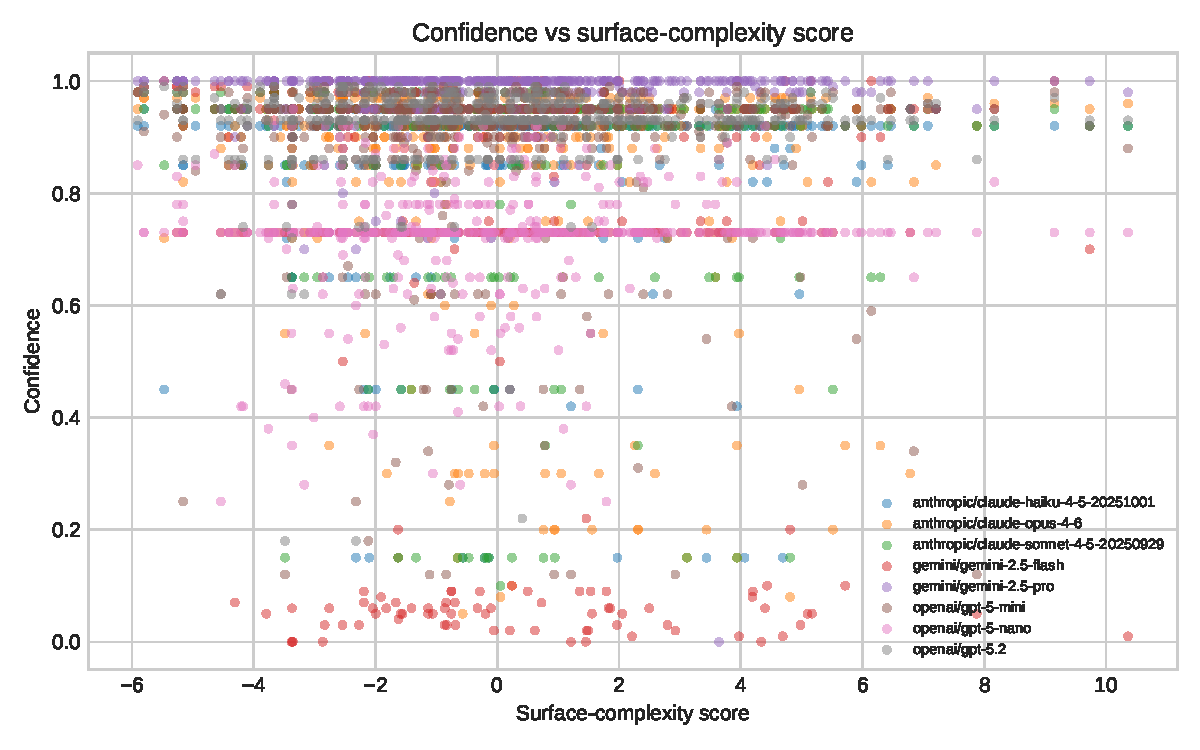
\includegraphics[width=0.95\linewidth]{figures/fig1_scatter_difficulty_vs_conf.pdf}}{}
\caption{Source-side surface-complexity proxy vs.\ self-reported confidence. The plot provides descriptive context only; the associated correlations in Table~\ref{tab:corr} are more interpretable than the raw scatter.}
\label{fig:conf_vs_complexity}
\end{figure}

\begin{figure}[t]
\centering
\IfFileExists{figures/fig2_reliability_diagram_overlay.pdf}{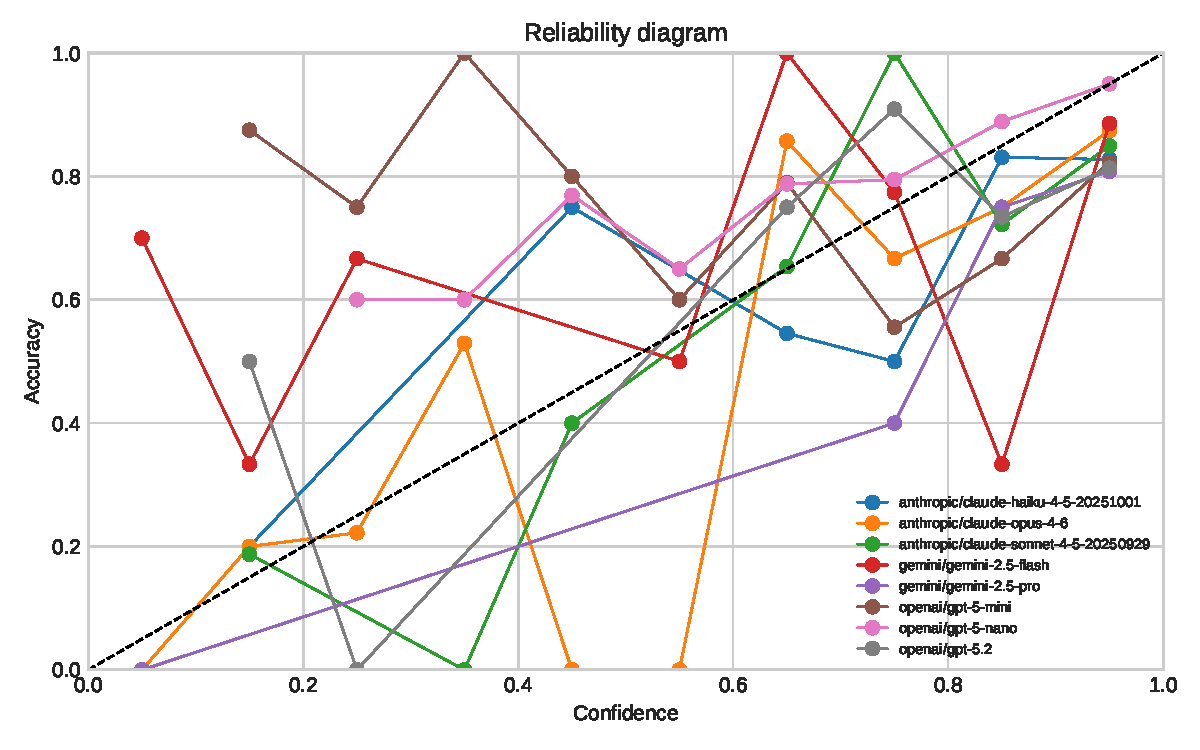
\includegraphics[width=0.95\linewidth]{figures/fig2_reliability_diagram_overlay.pdf}}{}
\caption{Overlaid reliability diagram with 10 bins. This figure is intended as a qualitative comparative view relative to the operational low-quality label rather than as the primary evidence for model ranking.}
\label{fig:reliability}
\end{figure}

\begin{figure}[t]
\centering
\IfFileExists{figures/fig3_mismatch_by_difficulty_bucket.pdf}{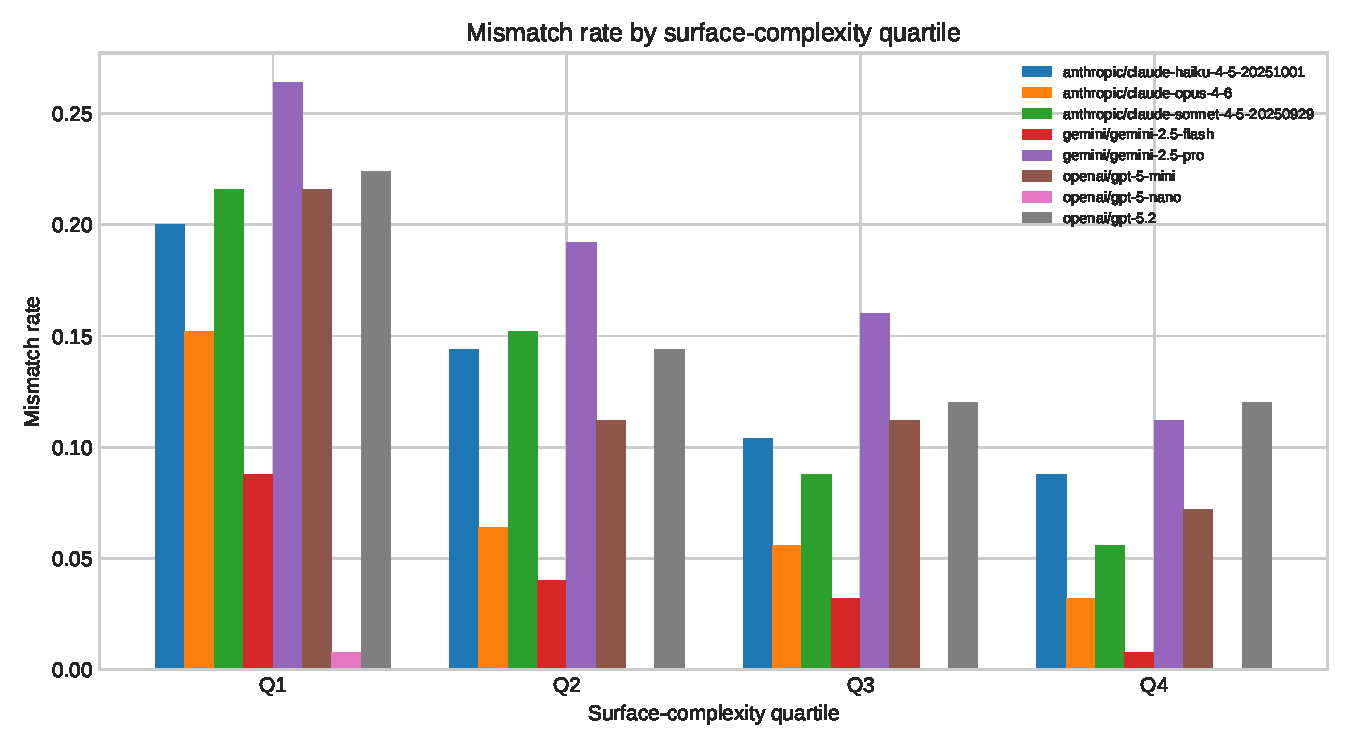
\includegraphics[width=0.95\linewidth]{figures/fig3_mismatch_by_difficulty_bucket.pdf}}{}
\caption{Mismatch@0.9 by source-side surface-complexity quartile. The figure is best interpreted as a secondary stratified view rather than as evidence for a strong difficulty effect.}
\label{fig:mismatch_by_complexity}
\end{figure}

\begin{figure}[t]
\centering
\IfFileExists{figures/fig4_efficiency_frontier.pdf}{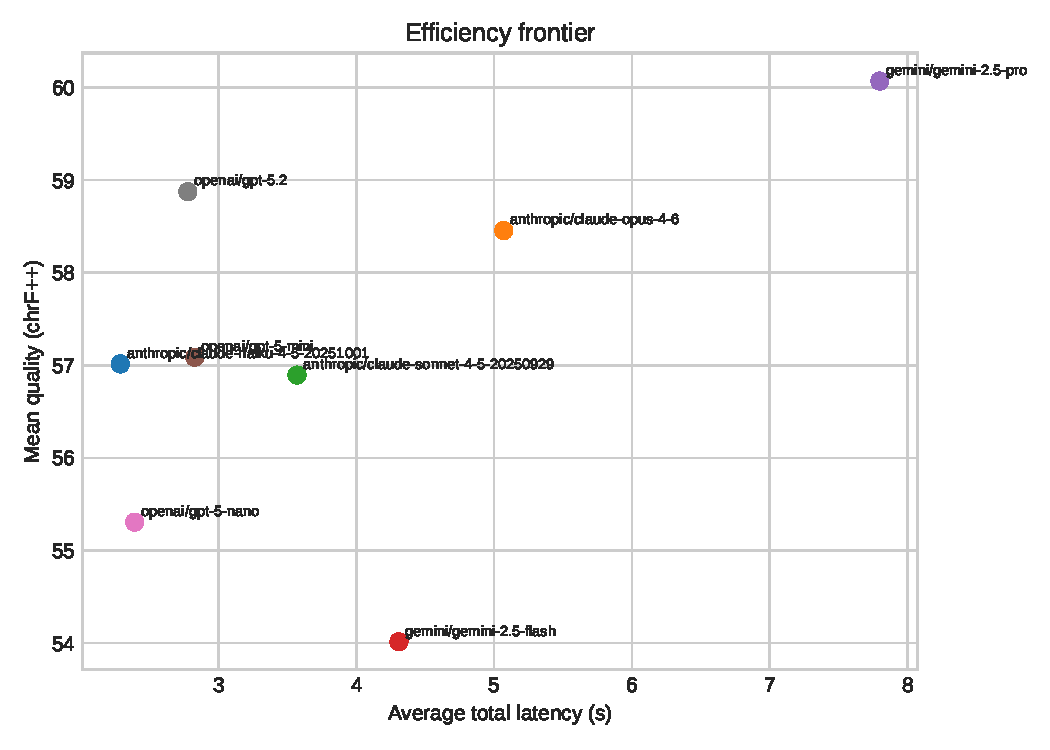
\includegraphics[width=0.75\linewidth]{figures/fig4_efficiency_frontier.pdf}}{}
\caption{Secondary quality--latency view across models. This figure provides supplementary deployment context and is not central to the paper's main claim about confidence portability.}
\label{fig:frontier}
\end{figure}

\section{Discussion and limitations}

\paragraph{Self-reported confidence scales are not directly comparable across providers.}
Confidence distributions differ sharply (Table~\ref{tab:main}). Gemini 2.5 Pro often outputs values at or near 1.00, whereas GPT-5-nano and Gemini 2.5 Flash are more conservative (median 0.73). As a result, a fixed threshold policy such as ``route to a human if confidence $< 0.9$'' would behave very differently across systems. Without calibration or per-provider tuning, that policy is not portable. This is the paper's main positive result. At the same time, low mismatch at a strict threshold should not be over-read as proof of a globally better confidence signal, because conservatism can also reduce the joint event $\Pr(\mathrm{low\mbox{-}quality} \wedge \mathrm{confidence}>\tau)$. Recent work on verbalized confidence supports this interpretation: black-box confidence scores can be informative, but they are highly sensitive to elicitation and often need explicit post-hoc calibration \citep{yang2024verbalizedconfidence,wang2024calibratingverbalized,ulmer-etal-2024-calibrating}.

\paragraph{The central construct is operational rather than semantic.}
The paper evaluates self-reported confidence against a chrF-based low-quality label rather than against human judgments of translation correctness. Under the within-model definition, low-quality prevalence is fixed at 20\% by construction, so the analysis compares how confidence aligns with a relative quality event within each model. This makes the results useful for controlled cross-provider comparison, but it also limits how strongly they can be interpreted as evidence about semantic correctness calibration. The manuscript is therefore strongest when it restricts its claim to portability under this protocol and target rather than to confidence faithfulness in a broader sense.

\paragraph{The source-side surface-complexity analysis should be read cautiously.}
Correlations between the source-side surface-complexity proxy and confidence are small (Table~\ref{tab:corr}), which is consistent with the idea that reported confidence is not derived directly from these surface features. The quartile-based mismatch plots show at most a modest descriptive tendency for several models rather than a uniform effect. The proxy is therefore useful mainly for coarse stratification, not for strong claims about translation difficulty. This is also a useful multilingual caution: recent confidence-estimation work shows that reliability can vary substantially across languages and prompting conditions, even when the same model family is used \citep{xue-etal-2025-mlingconf}.

\paragraph{Robustness to the low-quality definition.}
The main analysis defines low-quality cases as within-model bottom 20\% chrF. Appendix~\ref{app:robustness} shows that mismatch@0.9 remains qualitatively similar under the chrF-based low-quality definitions available in the released snapshot used for this paper (within-model bottom 20\% chrF and global bottom 20\% chrF). The ranking is not identical under every choice, but the qualitative gap between conservative and more aggressive confidence behavior remains.

\paragraph{What the supplementary mitigation does and does not show.}
The isotonic post-hoc analysis is encouraging in one limited sense: on a held-out split, provider-specific remapping often reduces ECE and lowers mismatch@0.9 relative to the same operational target. That makes provider-side mitigation more plausible for deployment. It does not, however, make the confidence scale portable. The learned remapping is model-specific, the gains are uneven, and one model (Claude Opus 4.6) shows worse held-out ECE after calibration. The right takeaway is therefore not that a lightweight calibration stage solves the problem, but that the problem can sometimes be mitigated only after treating each provider separately.

\paragraph{Practical implication.}
The strongest practical implication is not that self-reported confidence is useless, but that it should be treated as a provider-specific decision signal rather than as a portable probability. In settings where confidence is used for routing or abstention, the immediate remedies suggested by the present results are provider-specific threshold tuning, explicit post-hoc calibration, or the addition of an external evaluator layer rather than blind reuse of a shared confidence threshold across APIs. A stronger selective-prediction evaluation would require additional utility-oriented metrics or threshold sweeps, but the present evidence is already sufficient to reject the idea that one strict threshold transfers cleanly across providers in this setup.

\subsection{Limitations and threats to validity}
\textbf{Self-reported confidence.} The confidence signal comes from black-box APIs and may reflect provider-specific conventions or instruction-following behavior rather than calibrated probabilities. Because confidence is elicited after generating the translation and conditioned on that translation, it may also include post-hoc rationalization.

\textbf{Automatic metrics as a proxy for correctness.} The paper evaluates confidence against chrF-based operational low-quality labels rather than human judgments of correctness. These labels can disagree with human judgments and can overweight surface similarity. Stronger learned metrics such as COMET, BLEURT, and xCOMET often provide a better approximation to human assessment \citep{rei2020comet,sellam2020bleurt,guerreiro-etal-2024-xcomet,freitag-etal-2024-llms}. The supplementary robustness stage reduces this limitation only partially in the present environment, because COMET was unavailable and the pipeline therefore fell back to sentence-level BLEU. Human evaluation or learned-metric validation would still materially strengthen the claims.

\textbf{Selective utility is only partially observed.} ECE and mismatch@0.9 help characterize operating points under the chosen target, but they do not by themselves provide a full selective-prediction evaluation. In particular, low mismatch at a strict threshold can reflect either useful separation or simple reluctance to emit very high confidence. A fuller routing analysis would require additional coverage-aware metrics or threshold sweeps.

\textbf{Scope.} The study covers one language pair (English-to-German), one dataset (WMT17), one prompt protocol, one decoding/setup configuration, and 500 sampled sentences. Generalization to other language pairs, domains, prompt variants, and longer segments remains open.

\textbf{The source-side surface-complexity proxy is intentionally simple.} The proxy uses basic source-side features rather than a semantic or human-judged notion of difficulty. More linguistically informed features, learned QE signals, or human annotations could provide sharper stratification.

\textbf{Prompt sensitivity.} Prompts are standardized and temperature 0 is used throughout, but confidence elicitation can still be sensitive to wording and formatting constraints. This is consistent with recent evidence on verbalized confidence in LLMs \citep{yang2024verbalizedconfidence,wang2024calibratingverbalized,yona-etal-2024-large}. Systematic prompt-robustness experiments remain future work.

\section{Conclusion}

A standardized confidence-elicitation protocol was run for English-to-German MT across eight LLMs from three providers. Although mean chrF scores are relatively similar across models, ECE and the prevalence of high-confidence low-quality outputs vary widely relative to the operational chrF-based target used here. The strongest result is therefore comparative and practical: under this prompt protocol and evaluation setup, self-reported confidence should not be treated as a portable probability across providers, and a shared threshold does not produce comparable operating points across systems.

The source-side surface-complexity analysis provides only a coarse secondary view. Its relationship to confidence is weak, and it should not be interpreted as a validated measure of translation difficulty. The supplementary isotonic analysis shows that provider-specific post-hoc remapping can improve alignment to the operational target for most models, but that mitigation is itself non-portable and therefore does not change the central conclusion. Likewise, the secondary metric-robustness stage preserves the same qualitative cross-provider pattern in the current environment, although here the fallback metric is BLEU rather than a stronger learned metric. The most plausible next step motivated by these results is therefore to treat confidence as a signal that may still be useful, but only after provider-specific threshold tuning, explicit post-hoc calibration, or combination with stronger external evaluation layers. Recent work on uncertainty-aware MT evaluation and quality estimation points in this direction, including LLM-based MT evaluation \citep{qian-etal-2024-what}, black-box confidence calibration from generations alone \citep{ulmer-etal-2024-calibrating}, and confidence-aware QE models such as Early-Exit and Instant Confidence COMET \citep{zouhar-etal-2026-early}. The present results do not establish that the most conservative model is the most useful in general; they establish that fixed-threshold operating points are provider-dependent under the released protocol and target.

\section*{Reproducibility}
A reproducibility package accompanies the paper. The reported analysis was regenerated from the released repository snapshot with seed \textbf{123} on the WMT17 \texttt{en-de} test set sampled to \textbf{500} sentence pairs via \texttt{sacrebleu --echo}. The aggregated dataset contains \textbf{4{,}000} model outputs (\textbf{500/500} for each of eight models). The accompanying materials record the repository commit, configuration hash, and analysis timestamp used to regenerate the paper outputs. The same bash entrypoint can also run the supplementary calibration, secondary-metric, and metric-robustness stages without new provider API calls when the required artifacts already exist. End-to-end scripts, prompts, and generated tables and figures are included.

\bibliographystyle{plainnat}
\bibliography{references,added_refs}

\appendix
\section{Prompt templates used in the canonical runs}
\label{app:prompts}

All providers are instructed to return strict JSON only. OpenAI and Gemini use the wording shown below; Anthropic uses slightly shorter but schema-equivalent wording (``Return JSON with exactly one key \ldots''). The protocol is therefore standardized at the schema and task level rather than being literally identical word-for-word across providers. When provider outputs are malformed or missing required fields, the pipeline applies deterministic extraction and repair heuristics before downstream aggregation.

\subsection{Translation prompt}
\begin{verbatim}
SYSTEM: You are a helpful assistant. Output must be strict JSON.
USER: Translate English to German. Return ONLY one JSON object with exactly
this key: {"translation":"..."}. No explanations, no markdown, no code fences.
SOURCE: <English sentence>
\end{verbatim}

\subsection{Confidence prompt}
The prompt asks for ``translation correctness confidence'' because that is the elicited verbalized signal. The paper then evaluates that signal against an operational chrF-based low-quality label rather than against a human correctness judgment.

\begin{verbatim}
SYSTEM: You are a helpful assistant. Output must be strict JSON.
USER: Rate translation correctness confidence from 0 to 1. Return ONLY one
JSON object with exactly this key: {"confidence":0.73}. No explanations, no
markdown, no code fences.
SOURCE: <English sentence>
TRANSLATION: <German hypothesis>
\end{verbatim}

\section{Illustrative operational mismatch examples}
\label{app:examples}

The examples below are illustrative only. They are not used to establish semantic error and should not be read as evidence of semantic incorrectness by themselves. Overlap-based metrics can under-reward semantically adequate paraphrases, especially at the sentence level. These examples are therefore included only to visualize the high-confidence, low-chrF region under the paper's operational definitions. The full exported list is provided in \texttt{paper/top\_mismatch\_examples.md}.

\begin{table}[h]
\centering
\scriptsize
\setlength{\tabcolsep}{4pt}
\begin{tabular}{rcccp{0.62\linewidth}}
\toprule
id & bucket & conf & chrF & example (source / hypothesis / reference) \\
\midrule
110 & Q1 & 0.99 & 16.06 & However, volunteers are already aware of this. / Freiwillige sind sich dessen jedoch bereits bewusst. / Sensibilisiert seien die Helfer aber schon. \\
11 & Q1 & 0.98 & 33.49 & ``The benefits of the restructuring programme will only become visible after 5 years,'' he said. / ``Die Vorteile des Umstrukturierungsprogramms werden erst nach fünf Jahren sichtbar werden'', sagte er. / ``Die Früchte der Umstrukturierung sind aber auch nach 5 Jahren noch nicht zu sehen'', hieß es. \\
266 & Q1 & 0.99 & 39.95 & It is still apparently unclear who is behind the attacks. / Es ist offenbar immer noch unklar, wer hinter den Angriffen steckt. / Noch sei unklar, welche Gruppe hinter den Anschlägen stecke. \\
\bottomrule
\end{tabular}
\caption{Illustrative high-confidence, low-chrF cases from the GPT-5.2 export. These examples visualize the operational mismatch region used in the paper, but they are not evidence of semantic incorrectness by themselves and may include semantically acceptable paraphrases that receive low overlap scores.}
\end{table}

\section{Robustness analyses}
\label{app:robustness}

Table~\ref{tab:robustness} reports mismatch@0.9 under the two chrF-based low-quality definitions available in the released snapshot used for this paper: (i) within-model bottom 20\% chrF and (ii) global bottom 20\% chrF across all models. The ranking is not identical under the two definitions, but the broad separation between more conservative and more aggressive confidence behavior remains.

\begin{table}[t]
\centering
\small
\begin{tabular}{lcc}
\toprule
Model & Mismatch@0.9 (within-model chrF-q20) & Mismatch@0.9 (global chrF-q20) \\
\midrule
anthropic/claude-haiku-4-5-20251001 & 13.4\% & 13.4\% \\
anthropic/claude-opus-4-6 & 7.6\% & 6.4\% \\
anthropic/claude-sonnet-4-5-20250929 & 12.8\% & 14.2\% \\
gemini/gemini-2.5-flash & 4.2\% & 5.6\% \\
gemini/gemini-2.5-pro & 18.2\% & 12.6\% \\
openai/gpt-5-mini & 12.8\% & 14.6\% \\
openai/gpt-5-nano & 0.2\% & 0.8\% \\
openai/gpt-5.2 & 15.2\% & 11.8\% \\
\bottomrule
\end{tabular}
\caption{Appendix robustness comparison across chrF-based low-quality definitions at $\tau=0.9$.}
\label{tab:robustness}
\end{table}


Table~\ref{tab:metric_robustness} adds a second robustness view based on the strongest secondary metric available in the current environment. In the present regenerated run, COMET was unavailable and the pipeline fell back to sentence-level BLEU, so this appendix should be read as a conservative overlap-based cross-check rather than as learned-metric validation.

\end{document}
